% Created 2019-09-28 Sat 09:38
\documentclass[9pt, b5paper]{article}
\usepackage{fontspec}
\usepackage{graphicx}
\usepackage{xcolor}
\usepackage[slantfont,boldfont]{xeCJK}
\setCJKmainfont[BoldFont = Heiti SC, ItalicFont = STFangsong]{STSong}
\setCJKsansfont{STHeiti}
\setCJKmonofont{STFangsong}
\usepackage{multirow}
\usepackage{multicol}
\usepackage{float}
\usepackage{textcomp}
\usepackage{geometry}
\geometry{left=1.2cm,right=1.2cm,top=1.5cm,bottom=1.0cm}
\usepackage{algorithm}
\usepackage{algorithmic}
\usepackage{latexsym}
\usepackage{natbib}
\usepackage{listings}
\usepackage{minted}
\usepackage[xetex,colorlinks=true,CJKbookmarks=true,linkcolor=blue,urlcolor=blue,menucolor=blue]{hyperref}
\author{deepwaterooo}
\date{\today}
\title{Android Activity Fragment Lifecycle}
\hypersetup{
  pdfkeywords={},
  pdfsubject={},
  pdfcreator={Emacs 25.3.1 (Org mode 8.2.7c)}}
\begin{document}

\maketitle
\tableofcontents


\section{Activity与Fragment生命周期探讨}
\label{sec-1}
\begin{itemize}
\item \url{https://www.jianshu.com/p/1b3f829810a1}
\end{itemize}
\subsection{Activity生命周期探讨}
\label{sec-1-1}

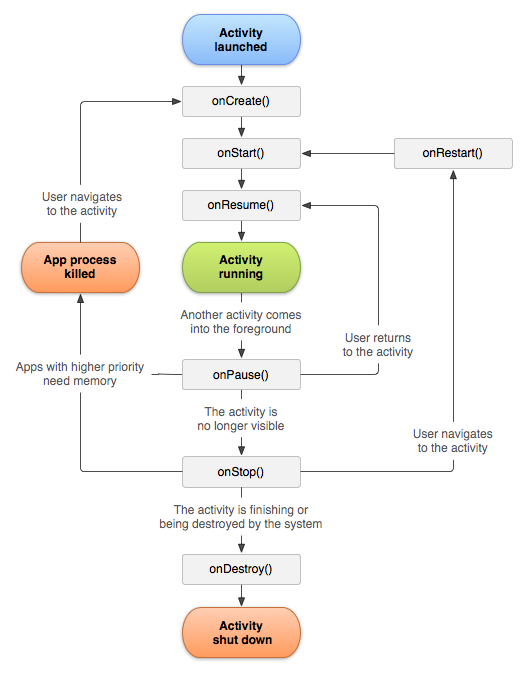
\includegraphics[width=.9\linewidth]{./pic/activityLifeCycle.png}
\subsubsection{Activity生命周期相关函数说明}
\label{sec-1-1-1}
\begin{itemize}
\item (1) onCreate()是activity正在被创建,也就是说此时的UI操作不会更新UI,比如setText()操作,所以此时在子线程调用setText()不会报线程错误。详解可见Android子线程更新View的探索,在这个方法内我们可以做一些初始化工作。
\item (2) onRestart()需要注意的是:activity正在重新启动,一般情况下,activity从不可见状态到可见状态,onRestart()才会被调用,但是一定要注意的是一般来说这是用户行为导致activity不可见的时候,此时变为可见的时候才会调用onRestart(),这里所说的用户行为就是用户按home键,或者进入“新”的activity。这样的操作会使activity先执行onPause(),后执行onStop(),这样回到这个activity会调用onRestart()。为什么我这里强调说用户行为导致的不可见状态,等下我会说。。。。
\item (3) onStart()的时候,activity才可见,但是没有出现在前台,无法与用户交互
\item (4) onResume()的时候,activity已经可见,并且出现在前台开始活动,与onStart()相比,activity都已经可见,但是onStart()的时候activity还在后台,onResume()才显示在前台
\item (5) onPause()主要注意的是:此时的activity正在被停止,接下来马上调用onStop()。特殊情况下快速回到该activity,onStop()不会执行,会去执行onResume()。
\begin{itemize}
\item 一般在这个生命周期内做存储数据、停止动画工作,但不能太耗时。
\item 为什么特殊强调呢,因为该activity的onPause()执行完了,才回去执行新的activity的onResume(),一旦耗时,必然会拖慢新的activity的显示。
\end{itemize}
\item (6) onStop():此时的activity即将停止。在这里可以做稍微重量级的操作,同样也不能耗时。
\item (7) onDestroy():此时的activity即将被回收,在这里会做一些回收工作和最终资源释放。
\end{itemize}
\subsubsection{他人总结}
\label{sec-1-1-2}
\begin{itemize}
\item \url{https://juejin.im/post/5a18f58651882531bb6c82e2}
\item 1. 打开一个全新的activityA:
\begin{itemize}
\item onCreate() ----> onStart() ----> onResume()
\end{itemize}
\item 2. 从activity A ----> activity B(全屏):
\begin{itemize}
\item activity A 先执行: onPause()
\item 然后activity B执行: onCreate() ----> onStart() ----> onResume()
\item activity A 再执行: onStop()
\end{itemize}
\item 3. 从activity A ----> activity B(非全屏):
\begin{itemize}
\item activity A先执行: onPause()
\item 然后activity B执行: onCreate() ----> onStart() ----> onResume()
\item \textbf{activity A不会执行onStop()}
\end{itemize}
\item 4. activity B(全屏)返回到 activity A:
\begin{itemize}
\item activity B 先执行: onPause()
\item activity A: onRestart ----> onStart() ----> onResume()
\item activity B再执行: onStop() ----> onDestory()
\end{itemize}
\item 5. activity B(非全屏)返回到activity A 
\begin{itemize}
\item activity B先执行: onPause()
\item activity A: onResume()
\item activity B再执行: onStop() ----> onDestory()
\end{itemize}
\item 6. activity B返回到activity A:
\begin{itemize}
\item 如果activityA已经被销毁,activityA会重新创建,执行: onCreate() ----> onStart() ----> onResume()
\item activityB的流程不变
\end{itemize}
\item 7. activity A按home键退居后台:
\begin{itemize}
\item 同2的流程: onPause()
\end{itemize}
\item 8. 再从home返回到activity A
\begin{itemize}
\item 同4的流程: onRestart ----> onStart() ----> onResume()
\end{itemize}
\end{itemize}

\subsubsection{Activity注意事项}
\label{sec-1-1-3}
\begin{itemize}
\item Activity中所有和状态相关的回调函数:

\includegraphics[width=.9\linewidth]{./pic/activityLifecyleCallbacks.png}
\item 在这里我会特别提出一个point,就是异常情况下activity被杀死,而后被重新创建的情况。

\begin{figure}[htb]
\centering
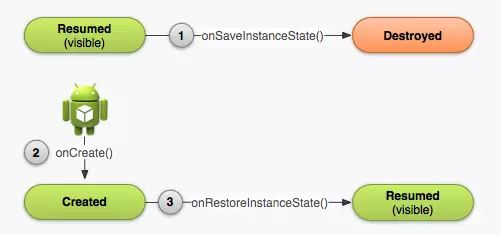
\includegraphics[width=.9\linewidth]{./pic/recreateActivity.png}
\caption{异常情况下activity的重建过程}
\end{figure}

\item 这张图非常重要,可以帮我们解决异常情况下activity如何正常回复的问题
\item 当系统停止activity时,它会调用onSaveInstanceState()(过程1),如果activity被销毁了,但是需要创建同样的实例,系统会把过程1中的状态数据传给onCreate()和onRestoreInstanceState(),所以我们要在onSaveInstanceState()内做保存参数的动作,在onRestoreInstanceState()做获取参数的动作。
\begin{minted}[linenos=true]{java}
// Save Activity State
static final String STATE_SCORE = "playerScore";
static final String STATE_LEVEL = "playerLevel";
@Override
public void onSaveInstanceState(Bundle savedInstanceState) {
    // Save the user's current game state
    savedInstanceState.putInt(STATE_SCORE, mCurrentScore);
    savedInstanceState.putInt(STATE_LEVEL, mCurrentLevel);
    // Always call the superclass so it can save the view hierarchy state
    super.onSaveInstanceState(savedInstanceState);
}
\end{minted}
\item 获取参数操作:
\begin{minted}[linenos=true]{java}
// onCreate() 方法
@Override
protected void onCreate(Bundle savedInstanceState) {
    super.onCreate(savedInstanceState); // Always call the superclass first

    // Check whether we're recreating a previously destroyed instance
    if (savedInstanceState != null) {
        // Restore value of members from saved state
        mCurrentScore = savedInstanceState.getInt(STATE_SCORE);
        mCurrentLevel = savedInstanceState.getInt(STATE_LEVEL);
    } else {
        // Probably initialize members with default values for a new instance
    }
}
\end{minted}
\item 也可以
\begin{minted}[linenos=true]{java}
// onRestoreInstanceState()方法
public void onRestoreInstanceState(Bundle savedInstanceState) {
    // Always call the superclass so it can restore the view hierarchy
    super.onRestoreInstanceState(savedInstanceState);
   
    // Restore state members from saved instance
    mCurrentScore = savedInstanceState.getInt(STATE_SCORE);
    mCurrentLevel = savedInstanceState.getInt(STATE_LEVEL);
}
\end{minted}
\end{itemize}

\subsubsection{一些特殊的方法}
\label{sec-1-1-4}
\begin{enumerate}
\item onWindowFocusChanged()
\label{sec-1-1-4-1}
\begin{itemize}
\item 在Activity窗口获得或失去焦点时被调用并且当Activity被创建时是在onResume之后被调用,当Activity被覆盖或者退居后台或者当前Activity退出时,它是在onPause之后被调用(在这个方法中可以view已经绘制完成,可以获取view的宽高等属性)
\end{itemize}
\item onSaveInstanceState()
\label{sec-1-1-4-2}
\begin{itemize}
\item (1)在Activity被覆盖或退居后台之后,系统资源不足将其杀死,此方法会被调用;
\item (2)在用户改变屏幕方向时,此方法会被调用;
\item (3)在当前Activity跳转到其他Activity或者按Home键回到主屏,自身退居后台时,此方法会被调用。
\item 第一种情况我们无法保证什么时候发生,系统根据资源紧张程度去调度;
\item 第二种是屏幕翻转方向时,系统先销毁当前的Activity,然后再重建一个新的,调用此方法时,我们可以保存一些临时数据;
\item 第三种情况系统调用此方法是为了保存当前窗口各个View组件的状态。
\item onSaveInstanceState的调用顺序是在onstop之前。(android3.0之前:在onPause之前调用,在3.0之后,在onPause之后调用)
\end{itemize}
\item onRestoreInstanceState()
\label{sec-1-1-4-3}
\begin{itemize}
\item 有的人说这个方法和onSaveInstanceState是一对,其实不然,
\item (1)在Activity被覆盖或退居后台之后,系统资源不足将其杀死,然后用户又回到了此Activity,此方法会被调用;
\item (2)在用户改变屏幕方向时,重建的过程中,此方法会被调用。
\item 我们可以重写此方法,以便可以恢复一些临时数据。
\item onRestoreInstanceState的调用顺序是在onStart之后。
\item 在当前Activity跳转到其他Activity或者按Home键回到主屏,自身退居后台时:onRestoreInstanceState不会调用,但是onSaveInstanceState会调用,这点就是区别
\end{itemize}
\end{enumerate}
\subsubsection{最后的总结}
\label{sec-1-1-5}
\begin{itemize}
\item 当Activity被系统撤销后重新建立时,保存以及恢复数据的函数调用顺序是:
\begin{itemize}
\item onSaveInstanceState(保存数据) ----> onCreate(恢复数据allstate) ----> onRestoryInstanceState(恢复数据HierarchyState)
\end{itemize}
\item 如果要取消切换屏幕方法重建activity,可以配置configChanges属性:当支持的最小sdk版本大于android4.0需要设置这个属性)
\begin{minted}[linenos=true]{java}
android:configChanges="keyboardHidden|orientation|screenSize(当支持的最小sdk版本大于android4.0需要设置这个属性)"
\end{minted}
\end{itemize}

\subsection{Fragment生命周期探讨}
\label{sec-1-2}
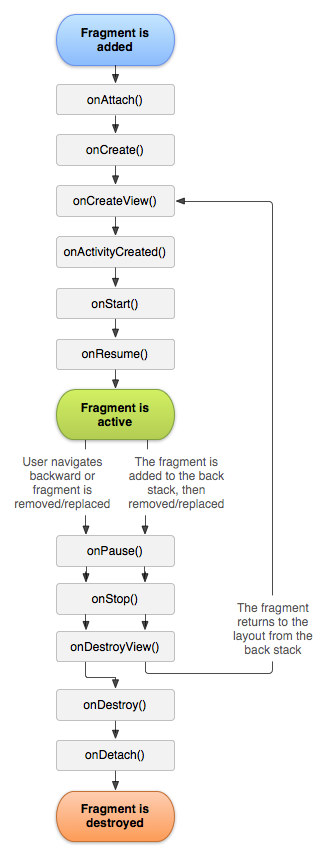
\includegraphics[width=.4\linewidth]{./pic/fragmentlifecycle.png}
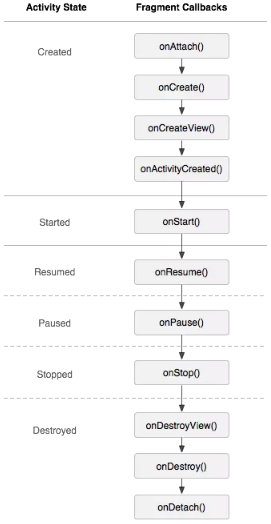
\includegraphics[width=.4\linewidth]{./pic/lifecyclecompare.png}

\begin{itemize}
\item Fragment基本类,生命周期如下:
\begin{minted}[linenos=true]{java}
void onAttach(Context context)
void onCreate(Bundle savedInstanceState)
View onCreateView(LayoutInflater inflater, ViewGroup container, Bundle savedInstanceState)
void onActivityCreated(Bundle savedInstanceState)
void onStart()
void onResume()
void onPause()
void onStop()
void onDestroyView()
void onDestroy()
void onDetach()
\end{minted}
\end{itemize}

\subsubsection{首先需要提出的一些points:}
\label{sec-1-2-1}
\begin{itemize}
\item Fragment是直接从Object继承的,而Activity是Context的子类。因此我们可以得出结论:Fragment不是Activity的扩展。但是与Activity一样,在我们使用Fragment的时候我们总会扩展Fragment(或者是她的子类),并可以通过子类更改她的行为。
\item 使用Fragment时,必要构建一个无参构造函数,系统会默认带。但一但写有参构造函数,就必要构建无参构造函数。一般来说我们传参数给Fragment,会通过bundle,而不会用构造方法传,代码如下:
\begin{minted}[linenos=true]{java}
public static MyFragment newInstance(int index){  
    MyFragment mf = new MyFragment();  
    Bundle args = new Bundle();  
    args.putInt("index",index);  
    mf.setArguments(args);  
    return mf;  
}
\end{minted}
\end{itemize}
\subsubsection{生命周期}
\label{sec-1-2-2}
\begin{itemize}
\item onAttach():onAttach()回调将在Fragment与其Activity关联之后调用。需要使用Activity的引用或者使用Activity作为其他操作的上下文,将在此回调方法中实现。
\begin{itemize}
\item 将Fragment附加到Activity以后,就无法再次调用setArguments()--除了在最开始,无法向初始化参数添加内容。
\end{itemize}
\item onCreate(Bundle savedInstanceState):此时的Fragment的onCreate()回调时,该fragmet还没有获得Activity的onCreate()已完成的通知,所以不能将依赖于Activity视图层次结构存在性的代码放入此回调方法中。在onCreate()回调方法中,我们应该尽量避免耗时操作。此时的bundle就可以获取到activity传来的参数
\begin{minted}[linenos=true]{java}
@Override
public void onCreate(Bundle savedInstanceState) {  
        super.onCreate(savedInstanceState);  
        Bundle args = getArguments();  
        if (args != null) {  
            mLabel = args.getCharSequence("label", mLabel);  
        }  
    }
\end{minted}
\item onCreateView()
\begin{minted}[linenos=true]{java}
onCreateView(LayoutInflater inflater, ViewGroup container, Bundle savedInstanceState)
\end{minted}
\begin{itemize}
\item 其中的Bundle为状态包与上面的bundle不一样。
\item 不要将视图层次结构附加到传入的ViewGroup父元素中,该关联会自动完成。如果在此回调中将碎片的视图层次结构附加到父元素,很可能会出现异常。
\item 这句话什么意思呢?就是不要把初始化的view视图主动添加到container里面,以为这会系统自带,所以inflate函数的第三个参数必须填false,而且不能出现container.addView(v)的操作。
\end{itemize}
\begin{minted}[linenos=true]{java}
View v = inflater.inflate(R.layout.hello_world, container, false);
\end{minted}
\item onActivityCreated()
\begin{itemize}
\item onActivityCreated()回调会在Activity完成其onCreate()回调之后调用。在调用onActivityCreated()之前,Activity的视图层次结构已经准备好了,这是在用户看到用户界面之前你可对用户界面执行的最后调整的地方。
\item 如果Activity和她的Fragment是从保存的状态重新创建的,此回调尤其重要,也可以在这里确保此Activity的其他所有Fragment已经附加到该Activity中了
\end{itemize}
\item Fragment与Activity相同生命周期调用:接下来的onStart(), onResume(), onPause(), onStop()回调方法将和Activity的回调方法进行绑定,也就是说与Activity中对应的生命周期相同,因此不做过多介绍。
\item onDestroyView():该回调方法在视图层次结构与Fragment分离之后调用。
\item onDestroy():不再使用Fragment时调用。(备注:Fragment仍然附加到Activity并任然可以找到,但是不能执行其他操作)
\item onDetach():Fragme生命周期最后回调函数,调用后,Fragment不再与Activity绑定,释放资源。
\end{itemize}

\subsubsection{Fragment每个生命周期方法的意义、作用}
\label{sec-1-2-3}
\begin{itemize}
\item onAttach()
\begin{itemize}
\item 执行该方法时,Fragment与Activity已经完成绑定,该方法有一个Activity类型的参数,代表绑定的Activity,这时候你可以执行诸如mActivity = activity的操作。
\end{itemize}
\item onCreate()
\begin{itemize}
\item 初始化Fragment。可通过参数savedInstanceState获取之前保存的值。
\end{itemize}
\item onCreateView()
\begin{itemize}
\item 初始化Fragment的布局。加载布局和findViewById的操作通常在此函数内完成,但是不建议执行耗时的操作,比如读取数据库数据列表。
\end{itemize}
\item onActivityCreated()
\begin{itemize}
\item 执行该方法时,与Fragment绑定的Activity的onCreate方法已经执行完成并返回,在该方法内可以进行与Activity交互的UI操作,所以在该方法之前Activity的onCreate方法并未执行完成,如果提前进行交互操作,会引发空指针异常。
\end{itemize}
\item onStart()
\begin{itemize}
\item 执行该方法时,Fragment由不可见变为可见状态。
\end{itemize}
\item onResume()
\begin{itemize}
\item 执行该方法时,Fragment处于活动状态,用户可与之交互。
\end{itemize}
\item onPause()
\begin{itemize}
\item 执行该方法时,Fragment处于暂停状态,但依然可见,用户不能与之交互。
\end{itemize}
\item onSaveInstanceState()
\begin{itemize}
\item 保存当前Fragment的状态。该方法会自动保存Fragment的状态,比如EditText键入的文本,即使Fragment被回收又重新创建,一样能恢复EditText之前键入的文本。
\end{itemize}
\item onStop()
\begin{itemize}
\item 执行该方法时,Fragment完全不可见。
\end{itemize}
\item onDestroyView()
\begin{itemize}
\item 销毁与Fragment有关的视图,但未与Activity解除绑定,依然可以通过onCreateView方法重新创建视图。通常在ViewPager+Fragment的方式下会调用此方法。
\end{itemize}
\item onDestroy()
\begin{itemize}
\item 销毁Fragment。通常按Back键退出或者Fragment被回收时调用此方法。
\end{itemize}
\item onDetach()
\begin{itemize}
\item 解除与Activity的绑定。在onDestroy方法之后调用。
\end{itemize}
\item setUserVisibleHint()
\begin{itemize}
\item 设置Fragment可见或者不可见时会调用此方法。在该方法里面可以通过调用getUserVisibleHint()获得Fragment的状态是可见还是不可见的,如果可见则进行懒加载操作。
\end{itemize}
\end{itemize}
\subsubsection{Fragment生命周期执行流程}
\label{sec-1-2-4}
\begin{itemize}
\item 1、Fragment创建
\begin{itemize}
\item setUserVisibleHint() ----> onAttach() ----> onCreate() ----> onCreateView() ----> onActivityCreated() ----> onStart() ----> onResume()
\end{itemize}
\item 2、Fragment变为不可见状态(锁屏、回到桌面、被Activity完全覆盖)
\begin{itemize}
\item onPause() ----> onSaveInstanceState() ----> onStop()
\end{itemize}
\item 3、Fragment变为部分可见状态(打开Dialog样式的Activity)
\begin{itemize}
\item onPause() ----> onSaveInstanceState()
\end{itemize}
\item 4、Fragment由不可见变为活动状态
\begin{itemize}
\item onStart() ----> OnResume()
\end{itemize}
\item 5、Fragment由部分可见变为活动状态
\begin{itemize}
\item onResume()
\end{itemize}
\item 6、Fragment退出
\begin{itemize}
\item onPause() ----> onStop() ----> onDestroyView() ----> onDestroy() ----> onDetach()
\item (注意退出不会调用onSaveInstanceState方法,因为是人为退出,没有必要再保存数据)
\end{itemize}
\item 7、Fragment被回收又重新创建
\begin{itemize}
\item 被回收执行: onPause() ----> onSaveInstanceState() ----> onStop() ----> onDestroyView() ----> onDestroy() ----> onDetach()
\item 重新创建执行: onAttach() ----> onCreate() ----> onCreateView() ----> onActivityCreated() ----> onStart() ----> onResume() ----> setUserVisibleHint()
\end{itemize}
\item 横竖屏切换
\begin{itemize}
\item 与Fragment被回收又重新创建一样。
\end{itemize}
\end{itemize}
\subsubsection{onHiddenChanged的回调时机}
\label{sec-1-2-5}
\begin{itemize}
\item 当使用add()+show(),hide()跳转新的Fragment时,旧的Fragment回调onHiddenChanged(),不会回调onStop()等生命周期方法,而新的Fragment在创建时是不会回调onHiddenChanged(),这点要切记。
\end{itemize}
\subsubsection{FragmentPagerAdapter+ViewPager的注意事项}
\label{sec-1-2-6}
\begin{itemize}
\item 1、 使用FragmentPagerAdapter+ViewPager时,切换回上一个Fragment页面时(已经初始化完毕),不会回调任何生命周期方法以及onHiddenChanged(),只有setUserVisibleHint(boolean isVisibleToUser)会被回调,所以如果你想进行一些懒加载,需要在这里处理。
\item 2、 在给ViewPager绑定FragmentPagerAdapter时,new FragmentPagerAdapter(fragmentManager)的FragmentManager,一定要保证正确,如果ViewPager是Activity内的控件,则传递getSupportFragmentManager(),如果是Fragment的控件中,则应该传递getChildFragmentManager()。只要记住ViewPager内的Fragments是当前组件的子Fragment这个原则即可。
\item 3、 你不需要考虑在“内存重启”的情况下,去恢复的Fragments的问题,因为FragmentPagerAdapter已经帮我们处理啦。
\end{itemize}
\subsubsection{setUserVisibleHint()不调用的问题}
\label{sec-1-2-7}
\begin{itemize}
\item 通常情况下都是因为PagerAdapter不是FragmentPagerAdapter造成的,FragmentPagerAdapter内部实现了对setUserVisibleHint()方法的调用,所以需要懒加载的结构最好使用FragmentPagerAdapter +Fragment的结构,少用PagerAdapter。
\end{itemize}

\subsubsection{Fragment注意事项}
\label{sec-1-2-8}
\begin{itemize}
\item 在使用Fragment时,我发现了一个金矿,那就是setRetainInstance()方法,此方法可以有效地提高系统的运行效率,对流畅性要求较高的应用可以适当采用此方法进行设置。
\item Fragment有一个非常强大的功能--就是可以在Activity重新创建时可以不完全销毁Fragment,以便Fragment可以恢复。在onCreate()方法中调用setRetainInstance(true/false)方法是最佳位置。当Fragment恢复时的生命周期如上图所示,注意图中的红色箭头。当在onCreate()方法中调用了setRetainInstance(true)后,Fragment恢复时会跳过onCreate()和onDestroy()方法,因此不能在onCreate()中放置一些初始化逻辑.
\end{itemize}
\section{Android Fragment 生命周期图}
\label{sec-2}
\begin{itemize}
\item \url{http://www.cnblogs.com/purediy/p/3276545.html}
\item Fragment与Activity生命周期对比图:
\end{itemize}

\subsection{生命周期分析}
\label{sec-2-1}
\subsubsection{当一个fragment被创建的时候(它会经历以下状态)}
\label{sec-2-1-1}
\begin{itemize}
\item onAttach()
\item onCreate()
\item onCreateView()
\item onActivityCreated()
\end{itemize}
\subsubsection{当这个fragment对用户可见的时候}
\label{sec-2-1-2}
\begin{itemize}
\item onStart()
\item onResume()
\end{itemize}
\subsubsection{当这个fragment进入“后台模式”的时候}
\label{sec-2-1-3}
\begin{itemize}
\item onPause()
\item onStop()
\end{itemize}
\subsubsection{当这个fragment被销毁了(或者持有它的activity被销毁了)}
\label{sec-2-1-4}
\begin{itemize}
\item onPause()
\item onStop()
\item onDestroyView()
\item onDestroy() // 本来漏掉类这个回调,感谢xiangxue336提出。
\item onDetach()
\end{itemize}
\subsubsection{就像activity一样,在以下的状态中,可以使用Bundle对象保存一个fragment的对象。}
\label{sec-2-1-5}
\begin{itemize}
\item onCreate()
\item onCreateView()
\item onActivityCreated()
\end{itemize}
\subsubsection{fragments的大部分状态都和activity很相似,但fragment有一些新的状态。}
\label{sec-2-1-6}
\begin{itemize}
\item onAttached() -- 当fragment被加入到activity时调用(在这个方法中可以获得所在的activity)。
\item onCreateView() -- 当activity要得到fragment的layout时,调用此方法,fragment在其中创建自己的layout(界面)。
\item onActivityCreated() -- 当activity的onCreated()方法返回后调用此方法
\item onDestroyView() -- 当fragment中的视图被移除的时候,调用这个方法。
\item onDetach() -- 当fragment和activity分离的时候,调用这个方法。
\item Notes:
\begin{itemize}
\item 一旦activity进入resumed状态(也就是running状态),你就可以自由地添加和删除fragment了。
\item 因此,只有当activity在resumed状态时,fragment的生命周期才能独立的运转,其它时候是依赖于activity的生命周期变化的。
\end{itemize}
\end{itemize}
% Emacs 25.3.1 (Org mode 8.2.7c)
\end{document}